\documentclass[a4paper,12 pt]{article}
\usepackage[T2A]{fontenc}
\usepackage[utf8]{inputenc}
\usepackage[english, russian]{babel}
\usepackage{geometry}
\usepackage{float}
\usepackage{amsfonts}
\usepackage{array}
\newcolumntype{C}[1]{>{\centering\arraybackslash}p{#1}}
 \geometry{
 a4paper,
 top=25mm,
 }
\usepackage{amsmath, amsfonts, amssymb, amsthm, mathtools, indentfirst, float, wrapfig}
\usepackage{graphicx}
\begin{document}
    \begin{titlepage}
    \begin{center}
        \vspace{4cm}
        \huge {\textbf{Отчет о выполнении лабораторной работы 1.3.1 }}
        {} \\
        \vspace{1cm}
        \Large {\textbf{Определение модуля Юнга на основе}} \\
        \Large {\textbf{исследования деформаций растяжения и изгиба}} \\
        \vspace{10cm}
        \begin{flushright}
        \begin{minipage}{.45\textwidth}
        \normalsize{\textbf{Студент:} Копытова Виктория Сергеевна}\\
        \textbf{Группа:} Б03-304\\
        \end{minipage}
        \end{flushright}   
    \end{center}
    \end{titlepage}
\newpage
 
\section{Аннотация}
\textbf{Цель работы:} экспериментально получить зависимость между напряжением и деформацией (закон Гука) для двух простейших напряженных состояний упругих тел: одноосного растяжения и чистого изгиба; по результатам измерений вычислить модуль Юнга.

\textbf{В работе используются:} в первой части - прибор Лермантова, проволока из исследуемого материала, зрительная труба со шкалой, набор грузов, микрометр, рулетка; во второй части - стойка для изгибания балки, индикатор для измерения величины прогиба, набор исследуемых стержней, грузы, линейка, штангенциркуль.
	

\section{Теоретические сведения}





\section{Ход работы}

\subsection{Определение модуля Юнга по измерениям растяжения проволоки}

Для определения модуля Юнга используется прибор Лермантова, схема которого изображена на рис. 1. Верхний конец проволоки П, изготовленной из исследуемого материала, прикреплен к консоли К, а нижний - к цилиндру, которым оканчивается шарнирный кронштейн Ш. На этот же цилиндр опирается рычаг г, связанный с зеркальцем 3. Таким образом, удлинение проволоки можно измерить по углу поворота зеркальца.
\begin{figure}[H]
    \centering
    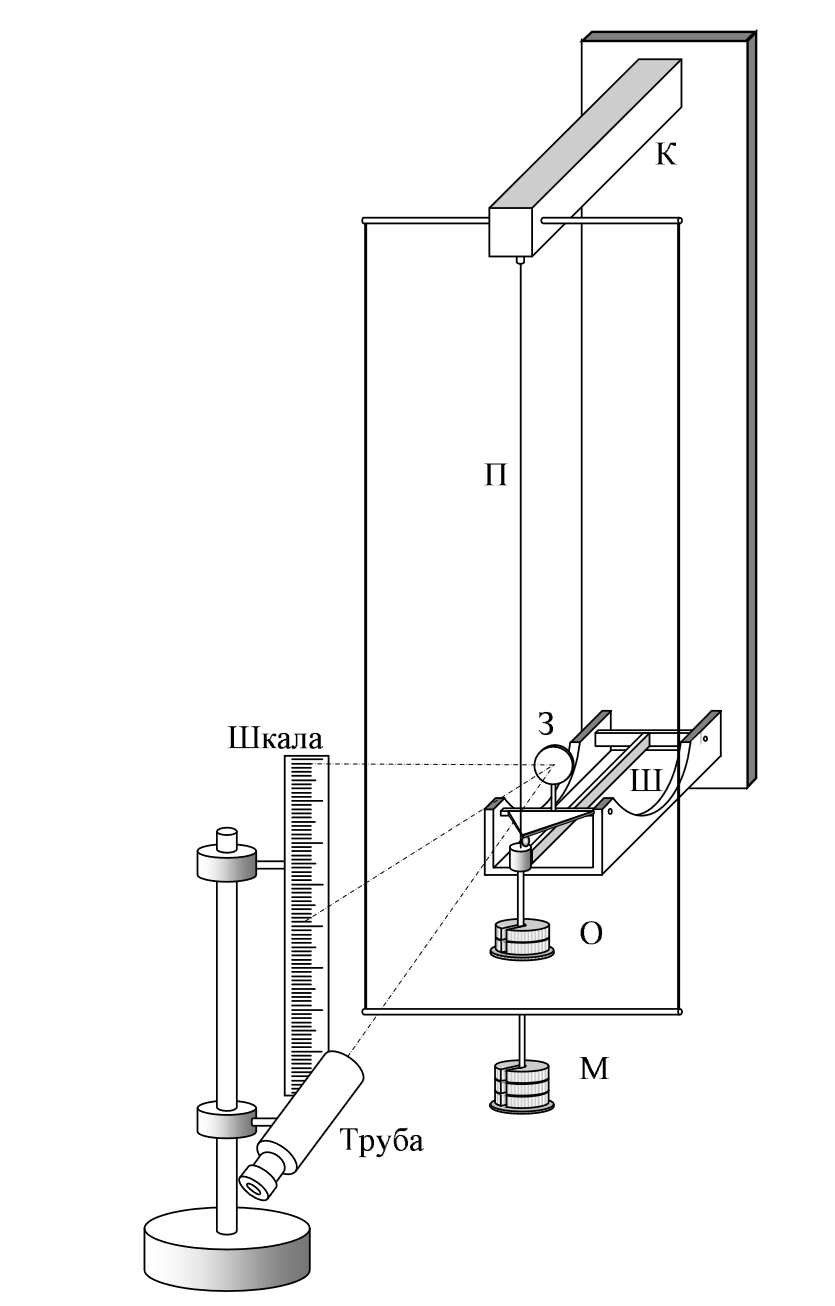
\includegraphics[scale = 0.4]{lermantov.png}
    \caption{Прибор Лермантова}
\end{figure}

Натяжение проволоки можно менять, перекладывая грузы с площадки М на площадку О и наоборот. Такая система позволяет исключить влияние деформации кронштейна К на точность измерений, так как нагрузка на нем все время остается постоянной.
Проволока П при отсутствии нагрузки всегда несколько изогнута, что не может не сказаться на результатах, особенно при небольших нагрузках. Проволока вначале не столько растягивается, сколько распрямляется.

\begin{enumerate}
    \item Параметры установки
    \begin{displaymath}
        d = (0.46 \pm 0.01) \quad \text{мм -- диаметр проволоки,}
    \end{displaymath}
    \begin{displaymath}
        r = 15 \quad \text{cм -- длина рычага,}
    \end{displaymath}
    \begin{displaymath}
        h = (143 \pm 0.1) \quad \text{cм -- расстояние от шкалы до зеркальца,}
    \end{displaymath}
    \begin{displaymath}
        L = (147.5 \pm 0.1) \quad \text{cм -- длина проволоки.}
    \end{displaymath}
    \item Площадь поперечного сечения проволоки
    \begin{displaymath}
        S = \pi \frac{d^2}{4} = 0.166 \quad \text{мм}^2
    \end{displaymath}
    \begin{displaymath}
        \sigma_S = S \cdot \sqrt{2 \Bigr( \frac{\sigma_d}{d} \Bigl)} = 0.005 \quad \text{мм}^2
    \end{displaymath}
    \item Направим зрительную трубу на зеркальце 3. При этом в трубу четко видно отражение шкалы в зеркальце. Тогда удлинение проволоки 
    \begin{displaymath}
        \Delta l = r \tan \varphi
    \end{displaymath}
    \begin{displaymath}
        \tan 2\varphi = \frac{n}{h} \approx 2\tan \varphi
    \end{displaymath}
    \begin{displaymath}
        \Delta l = \frac{nr}{2h}
    \end{displaymath}
    \begin{displaymath}
        \sigma_{\Delta l} = \Delta l\sqrt{\left( \dfrac{\sigma_{n}}{n}\right)^2 + \left(\dfrac{\sigma_d}{d}\right)^2+\left(\dfrac{\sigma_h}{h}\right)^2}
    \end{displaymath}
    \begin{figure}[H]
        \centering
        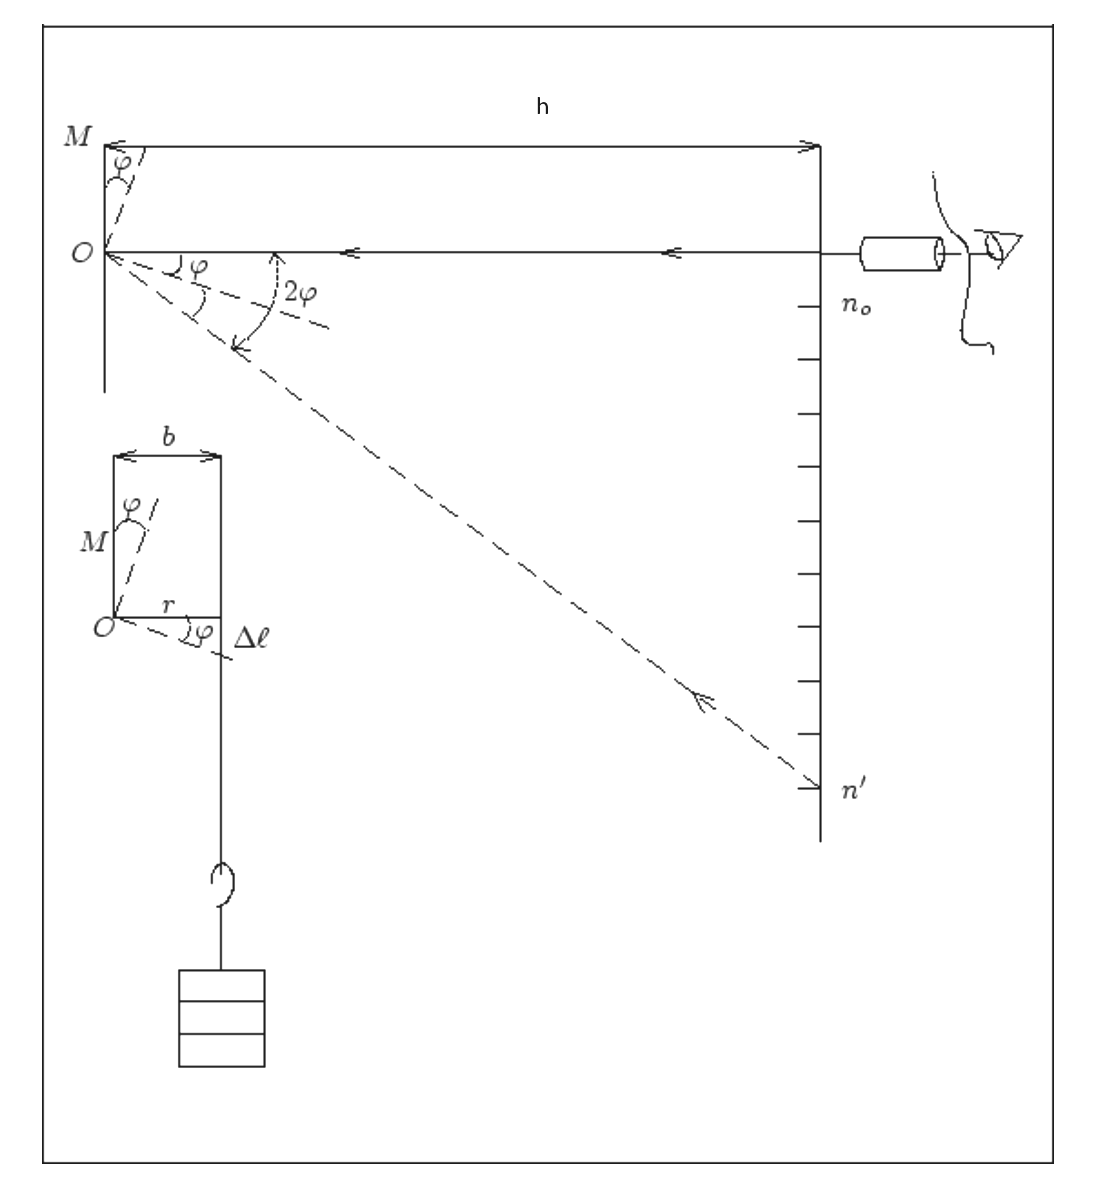
\includegraphics[scale = 0.5]{l.png}
        \caption{Вычисление удлинения проволоки}
    \end{figure}
    \item Оценим максимальную величину нагрузки, приняв разрушающее напряжение $\sigma_{\text{разр}} = 900 \quad \text{Н}/\text{мм}^2$. Тогда рабочее напряжение не должно превышать 30\% от величины разрушающего, а максимальная масса груза -- 4.57 кг.
    \item Проведём измерения при увеличении и при уменьшении нагрузки. Результаты занесём в таблицу 1.
    \begin{table}[H]
        \centering
        \begin{tabular}{|c|c|c|c|c|c|}
            \hline
            P, Н & 2.41 & 4.80 & 7.21 & 9.62 & 12.03 \\
            \hline
            $\Delta l$, мм & 0.142 & 0.320 & 0.488 & 0.640 & 0.776 \\
            \hline
            $\sigma_{\Delta l}$, мм & 0.004 & 0.007 & 0.011 & 0.014 & 0.017\\
            \hline
            \hline
            P, Н & 12.03 & 9.62 & 7.21 & 4.80 & 2.41 \\
            \hline
            $\Delta l$, мм & 0.776 & 0.635 & 0.488 & 0.315 & 0.142 \\
            \hline
            $\sigma_{\Delta l}$, мм & 0.017 & 0.014 & 0.011 & 0.007 & 0.004\\
            \hline
        \end{tabular}
        \caption{Удлинения проволоки}
    \end{table}
    По получнным данным построим графики, изображённые на рисунках 2-3.

    \begin{figure}[H]
        \centering
        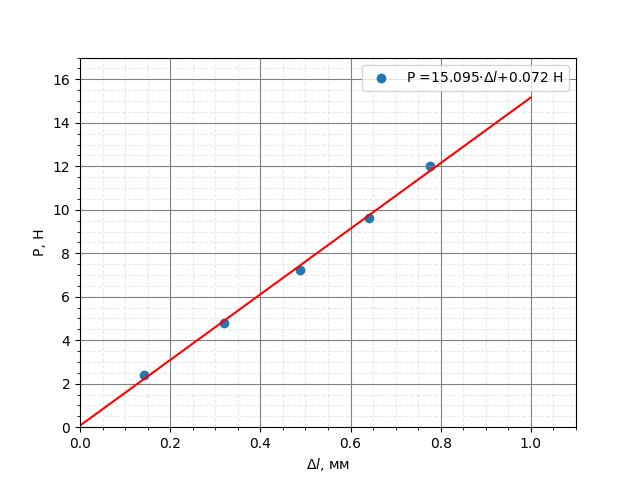
\includegraphics[scale = 0.7]{up.jpg}
        \caption{Увеличение нагрузки}
    \end{figure}

    \begin{figure}[H]
        \centering
        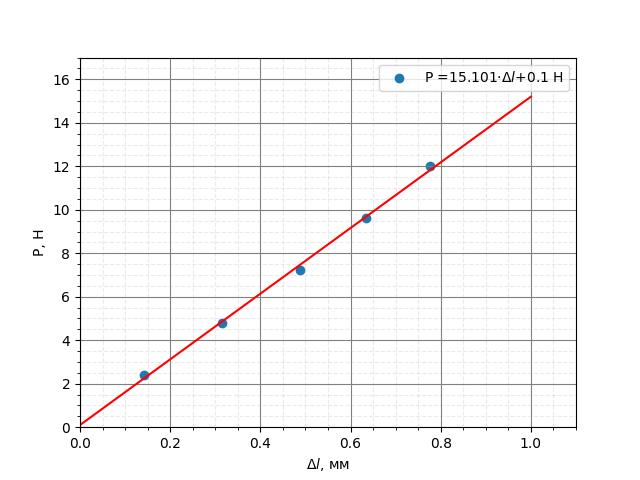
\includegraphics[scale = 0.7]{down.jpg}
        \caption{Уменьшение нагрузки}
    \end{figure}
    \item Вычислим модуль Юнга по формуле
    \begin{displaymath}
        E = \frac{\sigma}{\varepsilon} = \frac{P L}{S \Delta l} = k \frac{L}{S},
    \end{displaymath}
    где $k$ -- коэффициент наклона графика $P(\Delta l)$.
    \begin{displaymath}
        \sigma_E = E \cdot \sqrt{\left( \dfrac{\sigma_{k}}{k} \right)^2 + \left( \dfrac{\sigma_{S}}{S} \right)^2 + \left( \dfrac{\sigma_{L}}{L} \right)^2 }  
    \end{displaymath}

    Окончательный результат
    \begin{displaymath}
        E = (1.61 \pm 0.05) \cdot 10^{11} \quad \text{Па}
    \end{displaymath}

    Сравнение с табличными значениями позволяет предположить, что материал проволоки - стальной сплав.
\end{enumerate}


\subsection{Определение модуля Юнга по измерениям изгиба балки}

Экспериментальная установка состоит из прочной стойки с опорными призмами А и Б (рис. 5). На ребра призм опирается исследуемый стержень (балка) В. В середине стержня на призме Д поднешена площадка П с грузами. Измерять стрелу прогиба можно с помощью индикатора И, укрепляемого на отдельной штанге. Полный оборот большой стрелки индикатора соответствует 1 мм и одному делению малого циферблата.
\begin{figure}[H]
    \centering
    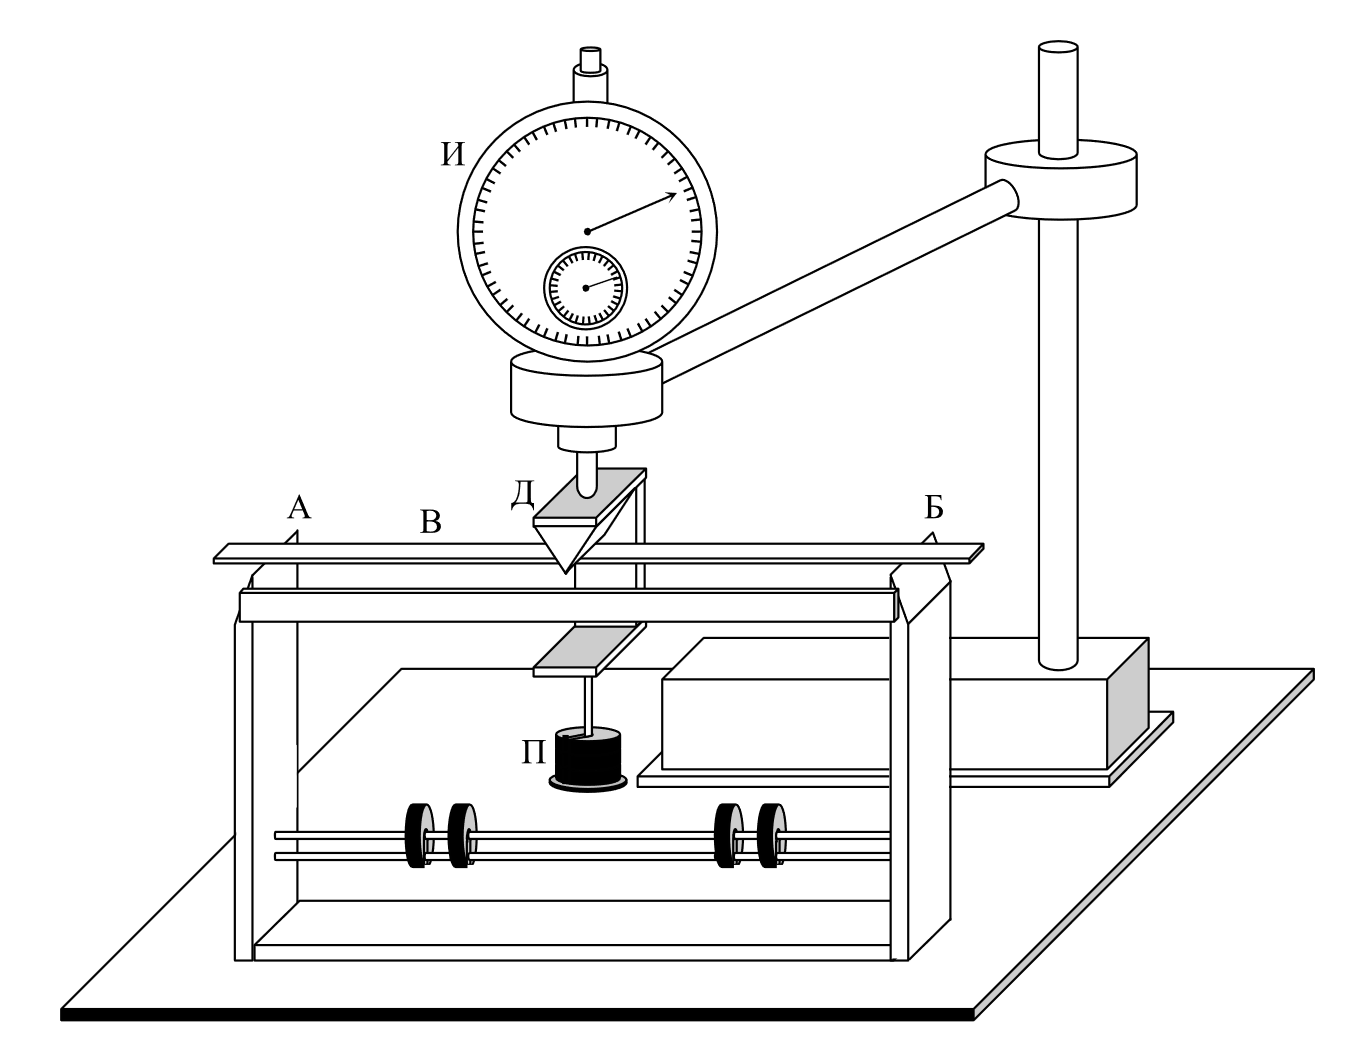
\includegraphics[scale = 0.4]{2.png}
    \caption{Схема уставовки для измерения модуля Юнга}
\end{figure}

\begin{enumerate}
    \item Параметры установки
    \begin{displaymath}
        l_{\text{АБ}} = (50 \pm 0.1) \quad \text{см}
    \end{displaymath}
    \begin{table}[H]
        \centering
        \begin{tabular}{|c|c|c|}
            \hline
            Материал стержня & Ширина, см & Высота, см \\
            \hline
            Медь & $2.18 \pm 0.01$ & $0.45 \pm 0.01$ \\
            \hline
            Дерево & $2.12 \pm 0.01$ & $0.95 \pm 0.01$ \\
            \hline
            Сталь & $2.10 \pm 0.01$ & $0.39 \pm 0.01$ \\
            \hline
        \end{tabular}
        \caption{Ширина и длина стержней}
    \end{table}
    \item Cнимем зависимость стрелы прогиба $y_{max}$ от величины нагрузки $P$. Измерения проделаем при возрастании и убывании нагрузки. Занесём результаты в таблицу.
    \begin{table}[H]
        \centering
        \begin{tabular}{|c|c|c|c|c||c|c|c|c|}
            \hline
            \multicolumn{9}{|c|}{Медь} \\
            \hline
            P, Н & 5.017 & 9.951 & 14.887 & 19.620 & 19.620 & 14.887 & 9.951 & 5.017 \\
            \hline
            $y_{max}$, мм & 0.72 & 1.48 & 2.21 & 2.97 & 2.97 & 2.26  & 1.44 & 0.68 \\
            \hline
            \hline
            \multicolumn{9}{|c|}{Дерево} \\
            \hline
            P, Н & 4.934 & 9.870 & 14.447 & 19.458 & 19.458 & 14.447 & 9.870 & 4.934 \\
            \hline
            $y_{max}$, мм & 0.61 & 1.24 & 1.78 & 2.59 & 2.59 & 1.82 & 1.26 & 0.62 \\
            \hline
            \hline
            \multicolumn{9}{|c|}{Cталь} \\
            \hline
            P, Н & 4.934 & 9.87 & 14.399 & 19.410 & 19.410 & 14.399 & 9.870 & 4.934 \\
            \hline
            $y_{max}$, мм & 0.68 & 1.31 & 1.97 & 2.56 & 2.56 & 2.01 & 1.3 & 0.69 \\
            \hline
        \end{tabular}
        \caption{Зависимость $y_{max}$ от нагрузки}
    \end{table}

    По полученным данным построим графики зависимости $P(y_{max})$.
    \begin{figure}[H]
        \centering
        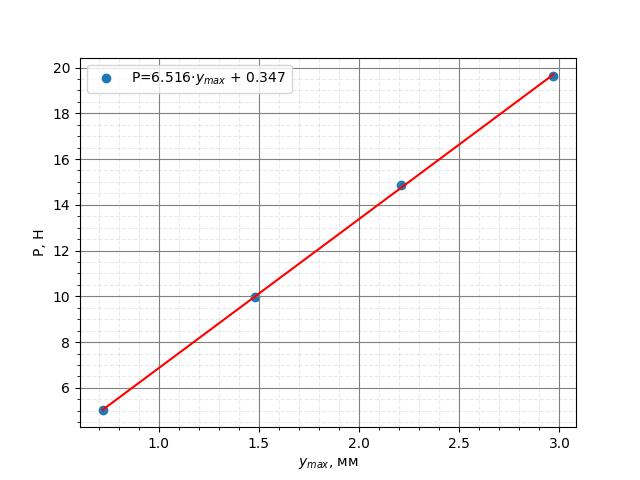
\includegraphics[scale = 0.7]{CuUp.jpg}
        \caption{Медь, увеличение нагрузки}
    \end{figure}
    \begin{figure}[H]
        \centering
        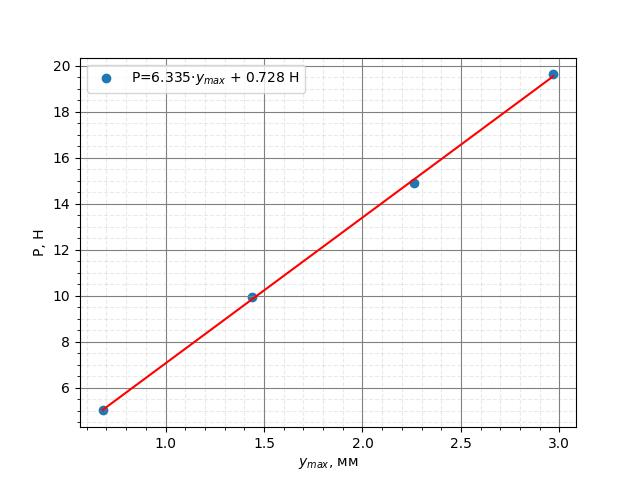
\includegraphics[scale=0.7]{CuDown.jpg}
        \caption{Медь, уменьшение нагрузки}
    \end{figure}

    \begin{figure}[H]
        \centering
        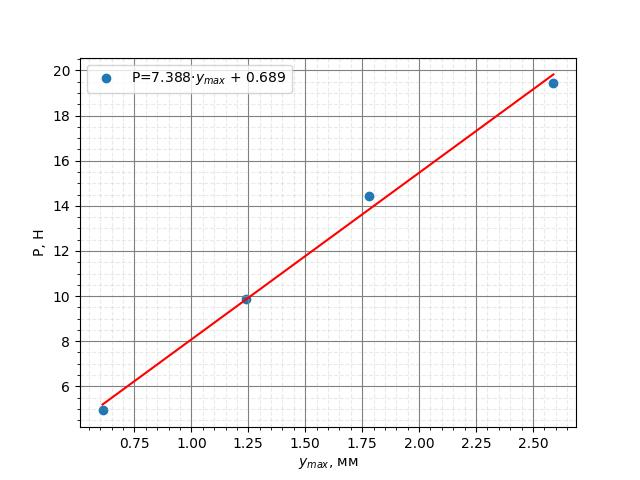
\includegraphics[scale = 0.7]{WoodUp.jpg}
        \caption{Дерево, увеличение нагрузки}
    \end{figure}
    \begin{figure}[H]
        \centering
        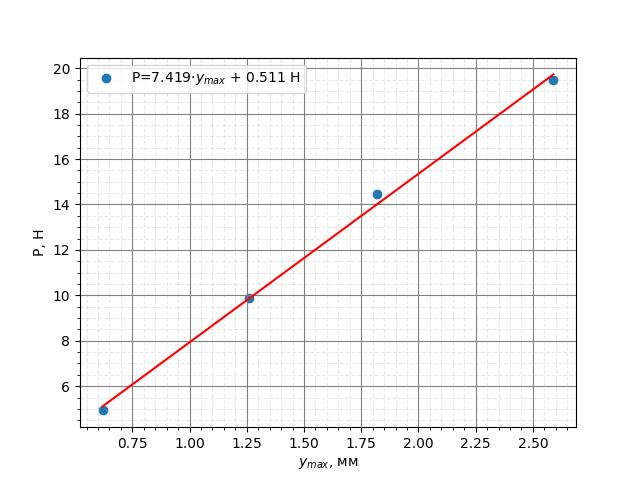
\includegraphics[scale=0.7]{WoodDown.jpg}
        \caption{Дерево, уменьшение нагрузки}
    \end{figure}

    \begin{figure}[H]
        \centering
        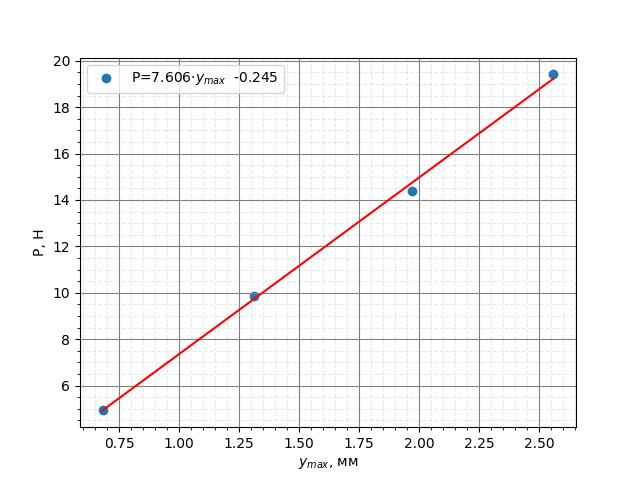
\includegraphics[scale = 0.7]{FeUp.jpg}
        \caption{Сталь, увеличение нагрузки}
    \end{figure}
    \begin{figure}[H]
        \centering
        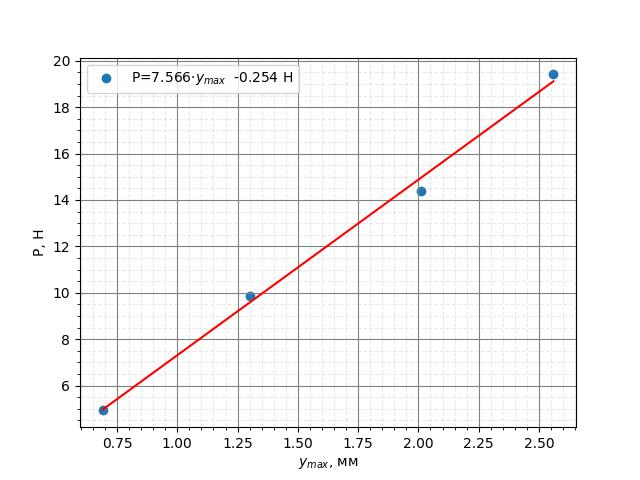
\includegraphics[scale=0.7]{FeDown.jpg}
        \caption{Сталь, уменьшение нагрузки}
    \end{figure}
    \item Вычислим модуль Юнга по формуле
    \begin{displaymath}
        E = \frac{Pl^3_{\text{АБ}}}{4ab^3 y_{max}},
    \end{displaymath}
    \begin{displaymath}
        \sigma_E = \sqrt{3 \left( \dfrac{\sigma_{l}}{l} \right)^2 + \left( \dfrac{\sigma_{P/y_{max}}}{P/y_{max}} \right)^2 + \left( \dfrac{\sigma_{a}}{a} \right)^2 + 3 \left( \dfrac{\sigma_{b}}{b} \right)^2}
    \end{displaymath}
    где $P/y_{max}$ -- средний коэффициент наклона графика зависимости $P(y_{max})$ при уменьшении и увеличении нагрузки.

    Окончательный результат
    \begin{table}[H]
        \centering
        \begin{tabular}{|c|c|}
            \hline
             Материал & Модуль Юнга, $10^{10}$ Па \\
             \hline
             Медь & $10.11 \pm 0.41$\\
             \hline
             Дерево & $19.03 \pm 0.41$\\
             \hline
             Сталь & $1.27 \pm 0.06$\\
             \hline
        \end{tabular}
        \caption{Модуль Юнга}
    \end{table}
\end{enumerate}
\section{Вывод}
В ходе работы двумя разными способами были измерены модули Юнга для различных материалов. Оба метода доказали свою применимость, позволив вычислить модули Юнга с точностью около 5\%. 
\end{document}


